\documentclass[12pt]{article}
\usepackage[utf8]{inputenc}
\usepackage{fullpage}
\usepackage{graphicx}
\usepackage{enumitem}
\usepackage{hanging}
\usepackage{lipsum}
\usepackage{svg}
\usepackage{amsmath}
\usepackage{xcolor}
\usepackage{soul}
\usepackage{color}
\usepackage[usenames,dvipsnames]{xcolor}
\usepackage{lastpage} % Required to determine the last page number for the footer
\usepackage{graphicx} % Required to insert images
\setlength\parindent{0pt} % Removes all indentation from paragraphs
\usepackage[most]{tcolorbox} % Required for boxes that split across pages
\usepackage{booktabs} % Required for better horizontal rules in tables
\usepackage{listings} % Required for insertion of code
\usepackage{etoolbox} % Required for if statements
\usepackage{geometry} % Required for adjusting page dimensions and margins
\usepackage{wrapfig}
\usepackage{algorithm}
\usepackage{algorithmic}
\usepackage{hyperref}
\usepackage{pdflscape}

\newcommand{\hlc}[2][yellow]{ {\sethlcolor{#1} \hl{#2}} }

\geometry{
	paper=a4paper, % Change to letterpaper for US letter
	top=3cm, % Top margin
	bottom=3cm, % Bottom margin
	left=2.5cm, % Left margin
	right=2.5cm, % Right margin
	headheight=14pt, % Header height
	footskip=1.4cm, % Space from the bottom margin to the baseline of the footer
	headsep=1.2cm, % Space from the top margin to the baseline of the header
	%showframe, % Uncomment to show how the type block is set on the page
}
\pagestyle{fancy} % Enable custom headers and footers



\title{IVR CW}
\author{Yannik Nelson}

\begin{document}
\maketitle
\tableofcontents \newpage

\section{Robot Vision}
\subsection{Joint State Estimation}
Here is the plot of my Joint State Estimations against their expected values:\newline
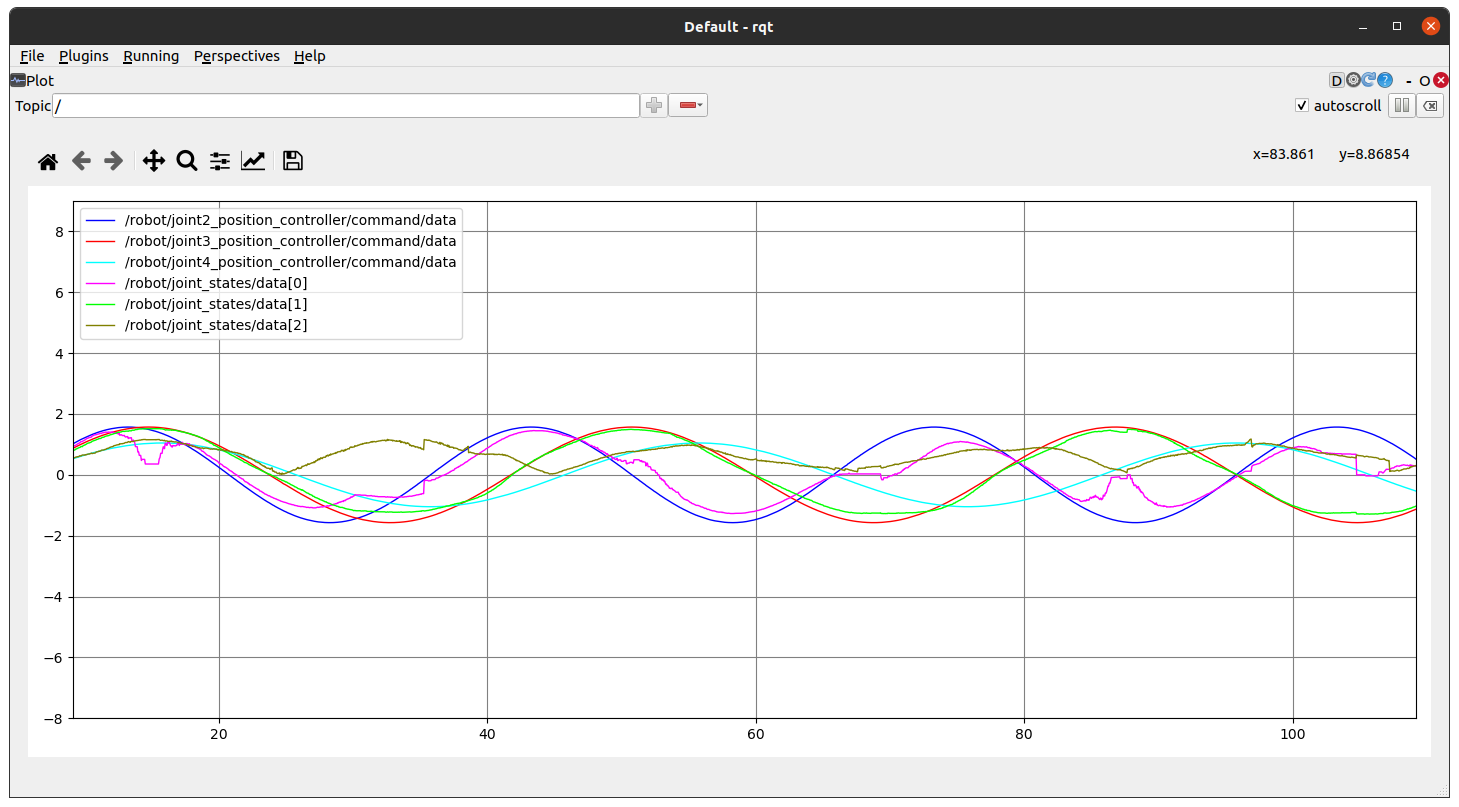
\includegraphics[width=\textwidth]{Joint_tracking_plus_one.png}
\subsection{Target Detection}
Here is the plot of the detected X Y and Z positions of the target plotted against the real values:\newline
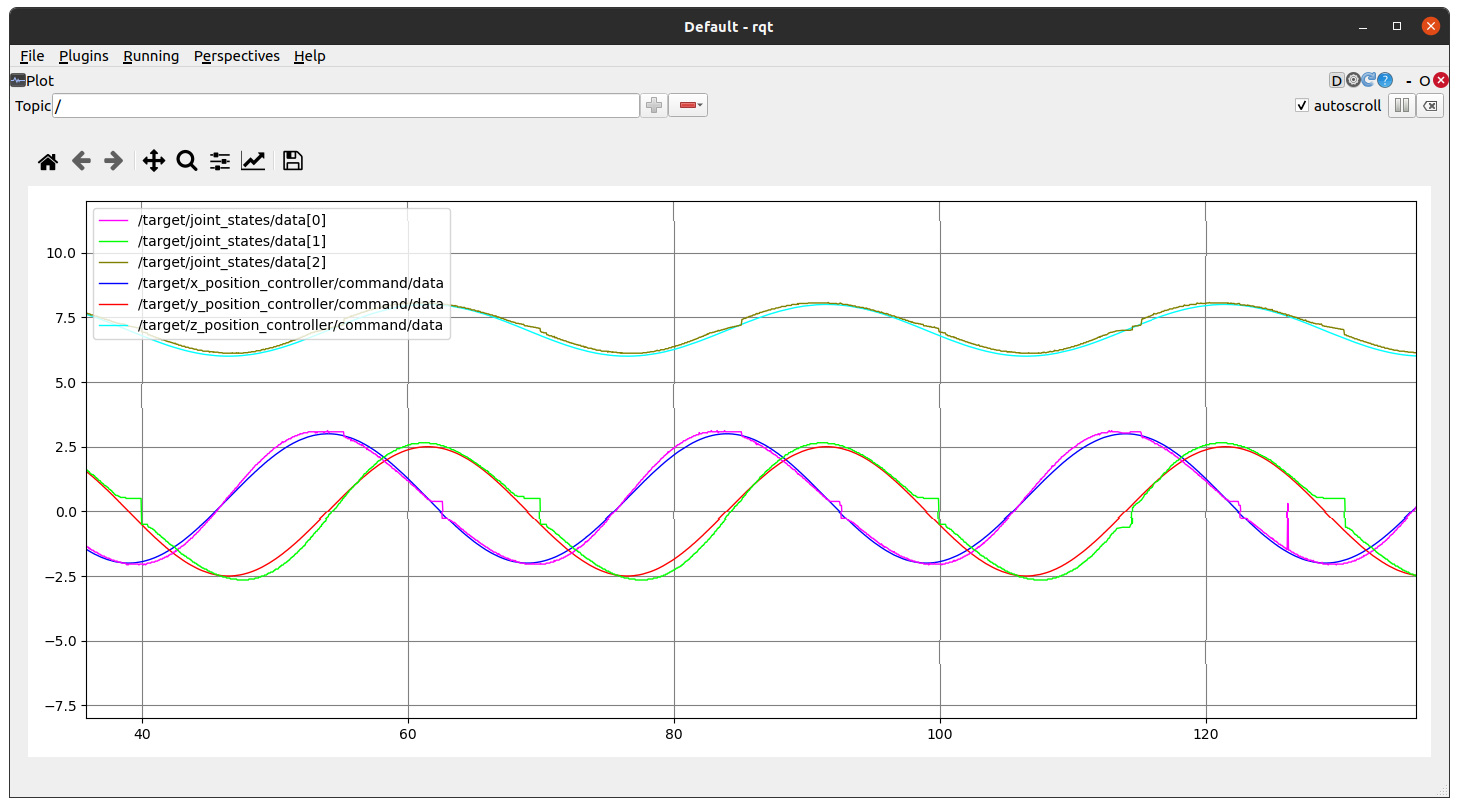
\includegraphics[width=\textwidth]{target_tacking_plus_one.png}
My algorithm works by taking in templates for the target and the box for each view and finding the contours for each at initialisation.
My algorithm then thresholds the images received from each camera, uses the cv2.findContours() function to find the contours and the cv2.matchShape() to check each contour against both the box and the target template contours, the result from these comparisons are checked and if the match to the target is greater than the match to the box then the moment for that contour is found, the center is extracted from that moment and that center is returned. If the algorithm doesn't isn't more sure either of the contours is the target then it will return the last saved position of the target in the respective view. I then find the x y z values from the position in the image as before. \newline
In the plot you can see flat parts and jumps in plots of the measured values. The spikes occur due to instances where partial obstruction of the wall or target causes the shape matching to confuse the target and the orange box. The Flat parts occur due to the obstruction of the target as well, except in these cases the shape matching 'catches' that the box is not the target and so doesn't change the measured position of the target until it's visible again.
\newpage
\section{Robot Control}
\subsection{Robot Kinematics}
D-H Table:
\begin{center}
    \begin{tabular}{c|c c c c}
         & \alpha & a & d & \theta \\ \hline
        1 & $\frac{\pi}{2}$ & 0 & 2.5 & $\theta_1 + \frac{\pi}{2}$\\
        2 & $\frac{\pi}{2}$&  0 & 0 & $\theta_2 + \frac{\pi}{2}$\\
        3 & $-\frac{\pi}{2}$ & 3.5 & 0 & \theta_3 \\
        4 & 0 & 3 & 0 & \theta_4\\
    \end{tabular}
\end{center}\newline
\begin{center}
    A_1^0 = $\left[\begin{matrix}c{\left(\theta_{1} + \frac{\pi}{2}\right)} & - s{\left(\theta_{1} + \frac{\pi}{2}\right)} & 0 & 0\\s{\left(\theta_{1} + \frac{\pi}{2}\right)} & c{\left(\theta_{1} + \frac{\pi}{2}\right)} & 0 & 0\\0 & 0 & 1 & 0\\0 & 0 & 0 & 1\end{matrix}\right]$$\left[\begin{matrix}1 & 0 & 0 & 0\\0 & 1 & 0 & 0\\0 & 0 & 1 & 2.5\\0 & 0 & 0 & 1\end{matrix}\right]$$\left[\begin{matrix}1 & 0 & 0 & 0\\0 & 1 & 0 & 0\\0 & 0 & 1 & 0\\0 & 0 & 0 & 1\end{matrix}\right]$$\left[\begin{matrix}1 & 0 & 0 & 0\\0 & c{\left(\frac{\pi}{2} \right)} & - s{\left(\frac{\pi}{2} \right)} & 0\\0 & s{\left(\frac{\pi}{2} \right)} & c{\left(\frac{\pi}{2} \right)} & 0\\0 & 0 & 0 & 1\end{matrix}\right]$\newline
    = $\left[\begin{matrix}- s{\left(\theta_{1} \right)} & 0 & c{\left(\theta_{1} \right)} & 0\\c{\left(\theta_{1} \right)} & 0 & s{\left(\theta_{1} \right)} & 0\\0 & 1 & 0 & 2.5\\0 & 0 & 0 & 1\end{matrix}\right]$\newline\newline
    
    A_2^1 = $\left[\begin{matrix}c{\left(\theta_{2} + \frac{\pi}{2}\right)} & - s{\left(\theta_{2} + \frac{\pi}{2}\right)} & 0 & 0\\s{\left(\theta_{2} + \frac{\pi}{2}\right)} & c{\left(\theta_{2} + \frac{\pi}{2}\right)} & 0 & 0\\0 & 0 & 1 & 0\\0 & 0 & 0 & 1\end{matrix}\right]$$\left[\begin{matrix}1 & 0 & 0 & 0\\0 & 1 & 0 & 0\\0 & 0 & 1 & 0\\0 & 0 & 0 & 1\end{matrix}\right]$$\left[\begin{matrix}1 & 0 & 0 & 0\\0 & 1 & 0 & 0\\0 & 0 & 1 & 0\\0 & 0 & 0 & 1\end{matrix}\right]$$\left[\begin{matrix}1 & 0 & 0 & 0\\0 & c{\left(\frac{\pi}{2} \right)} & - s{\left(\frac{\pi}{2} \right)} & 0\\0 & s{\left(\frac{\pi}{2} \right)} & c{\left(\frac{\pi}{2} \right)} & 0\\0 & 0 & 0 & 1\end{matrix}\right]$\newline
    $\left[\begin{matrix}- s{\left(\theta_{2} \right)} & 0 & c{\left(\theta_{2} \right)} & 0\\c{\left(\theta_{2} \right)} & 0 & s{\left(\theta_{2} \right)} & 0\\0 & 1 & 0 & 0\\0 & 0 & 0 & 1\end{matrix}\right]$\newline\newline
    
    A_3^2 = $\left[\begin{matrix}c{\left(\theta_{3}\right)} & - s{\left(\theta_{3} \right)} & 0 & 0\\s{\left(\theta_{3} \right)} & c{\left(\theta_{3} \right)} & 0 & 0\\0 & 0 & 1 & 0\\0 & 0 & 0 & 1\end{matrix}\right]$$\left[\begin{matrix}1 & 0 & 0 & 0\\0 & 1 & 0 & 0\\0 & 0 & 1 & 0\\0 & 0 & 0 & 1\end{matrix}\right]$$\left[\begin{matrix}1 & 0 & 0 & 3.5\\0 & 1 & 0 & 0\\0 & 0 & 1 & 0\\0 & 0 & 0 & 1\end{matrix}\right]$$\left[\begin{matrix}1 & 0 & 0 & 0\\0 & c{\left(-\frac{\pi}{2} \right)} & - s{\left(-\frac{\pi}{2} \right)} & 0\\0 & s{\left(-\frac{\pi}{2} \right)} & c{\left(-\frac{\pi}{2} \right)} & 0\\0 & 0 & 0 & 1\end{matrix}\right]$\newline
    = $\left[\begin{matrix}c{\left(\theta_{3} \right)} & 0 & - s{\left(\theta_{3} \right)} & 3.5 c{\left(\theta_{3} \right)}\\s{\left(\theta_{3} \right)} & 0 & c{\left(\theta_{3} \right)} & 3.5 s{\left(\theta_{3} \right)}\\0 & -1 & 0 & 0\\0 & 0 & 0 & 1\end{matrix}\right]$\newline\newline
    
    A_4^3 = $\left[\begin{matrix}c{\left(\theta_{4}\right)} & - s{\left(\theta_{4} \right)} & 0 & 0\\s{\left(\theta_{4} \right)} & c{\left(\theta_{4} \right)} & 0 & 0\\0 & 0 & 1 & 0\\0 & 0 & 0 & 1\end{matrix}\right]$$\left[\begin{matrix}1 & 0 & 0 & 0\\0 & 1 & 0 & 0\\0 & 0 & 1 & 0\\0 & 0 & 0 & 1\end{matrix}\right]$$\left[\begin{matrix}1 & 0 & 0 & 3\\0 & 1 & 0 & 0\\0 & 0 & 1 & 0\\0 & 0 & 0 & 1\end{matrix}\right]$$\left[\begin{matrix}1 & 0 & 0 & 0\\0 & 1 & 0 & 0\\0 & 0 & 1 & 0\\0 & 0 & 0 & 1\end{matrix}\right]$\newline
    = $\left[\begin{matrix}c{\left(\theta_{4} \right)} & - s{\left(\theta_{4} \right)} & 0 & 3 c{\left(\theta_{4} \right)}\\s{\left(\theta_{4} \right)} & c{\left(\theta_{4} \right)} & 0 & 3 s{\left(\theta_{4} \right)}\\0 & 0 & 1 & 0\\0 & 0 & 0 & 1\end{matrix}\right]$
\end{center}

\begin{landscape}
\begin{center}
\begin{tabular}{c}
     A_1^0A_2^1A_3^2A_4^3 = $\left[\begin{matrix}\left(s{\left(\theta_{1} \right)} s{\left(\theta_{2} \right)} c{\left(\theta_{3} \right)} + s{\left(\theta_{3} \right)} c{\left(\theta_{1} \right)}\right) c{\left(\theta_{4} \right)} + s{\left(\theta_{1} \right)} s{\left(\theta_{4} \right)} c{\left(\theta_{2} \right)} & - \left(s{\left(\theta_{1} \right)} s{\left(\theta_{2} \right)} c{\left(\theta_{3} \right)} + s{\left(\theta_{3} \right)} c{\left(\theta_{1} \right)}\right) s{\left(\theta_{4} \right)} + s{\left(\theta_{1} \right)} c{\left(\theta_{2} \right)} c{\left(\theta_{4} \right)}\\\left(s{\left(\theta_{1} \right)} s{\left(\theta_{3} \right)} - s{\left(\theta_{2} \right)} c{\left(\theta_{1} \right)} c{\left(\theta_{3} \right)}\right) c{\left(\theta_{4} \right)} - s{\left(\theta_{4} \right)} c{\left(\theta_{1} \right)} c{\left(\theta_{2} \right)} & - \left(s{\left(\theta_{1} \right)} s{\left(\theta_{3} \right)} - s{\left(\theta_{2} \right)} c{\left(\theta_{1} \right)} c{\left(\theta_{3} \right)}\right) s{\left(\theta_{4} \right)} - c{\left(\theta_{1} \right)} c{\left(\theta_{2} \right)} c{\left(\theta_{4} \right)}\\- s{\left(\theta_{2} \right)} s{\left(\theta_{4} \right)} + c{\left(\theta_{2} \right)} c{\left(\theta_{3} \right)} c{\left(\theta_{4} \right)} & - s{\left(\theta_{2} \right)} c{\left(\theta_{4} \right)} - s{\left(\theta_{4} \right)} c{\left(\theta_{2} \right)} c{\left(\theta_{3} \right)}\\0 & 0\end{matrix}\right.$\\\\
     $\left.\begin{matrix}- s{\left(\theta_{1} \right)} s{\left(\theta_{2} \right)} s{\left(\theta_{3} \right)} + c{\left(\theta_{1} \right)} c{\left(\theta_{3} \right)} & 3 \left(s{\left(\theta_{1} \right)} s{\left(\theta_{2} \right)} c{\left(\theta_{3} \right)} + s{\left(\theta_{3} \right)} c{\left(\theta_{1} \right)}\right) c{\left(\theta_{4} \right)} + 3.5 s{\left(\theta_{1} \right)} s{\left(\theta_{2} \right)} c{\left(\theta_{3} \right)} + 3 s{\left(\theta_{1} \right)} s{\left(\theta_{4} \right)} c{\left(\theta_{2} \right)} + 3.5 s{\left(\theta_{3} \right)} c{\left(\theta_{1} \right)}\\s{\left(\theta_{1} \right)} c{\left(\theta_{3} \right)} + s{\left(\theta_{2} \right)} s{\left(\theta_{3} \right)} c{\left(\theta_{1} \right)} & 3 \left(s{\left(\theta_{1} \right)} s{\left(\theta_{3} \right)} - s{\left(\theta_{2} \right)} c{\left(\theta_{1} \right)} c{\left(\theta_{3} \right)}\right) c{\left(\theta_{4} \right)} + 3.5 s{\left(\theta_{1} \right)} s{\left(\theta_{3} \right)} - 3.5 s{\left(\theta_{2} \right)} c{\left(\theta_{1} \right)} c{\left(\theta_{3} \right)} - 3 s{\left(\theta_{4} \right)} c{\left(\theta_{1} \right)} c{\left(\theta_{2} \right)}\\- s{\left(\theta_{3} \right)} c{\left(\theta_{2} \right)} & - 3 s{\left(\theta_{2} \right)} s{\left(\theta_{4} \right)} + 3 c{\left(\theta_{2} \right)} c{\left(\theta_{3} \right)} c{\left(\theta_{4} \right)} + 3.5 c{\left(\theta_{2} \right)} c{\left(\theta_{3} \right)} + 2.5\\0 & 1\end{matrix}\right]$\\\\
so:\\
$\left[\begin{matrix}3 \left(s{\left(\theta_{1} \right)} s{\left(\theta_{2} \right)} c{\left(\theta_{3} \right)} + s{\left(\theta_{3} \right)} c{\left(\theta_{1} \right)}\right) c{\left(\theta_{4} \right)} + 3.5 s{\left(\theta_{1} \right)} s{\left(\theta_{2} \right)} c{\left(\theta_{3} \right)} + 3 s{\left(\theta_{1} \right)} s{\left(\theta_{4} \right)} c{\left(\theta_{2} \right)} + 3.5 s{\left(\theta_{3} \right)} c{\left(\theta_{1} \right)}\\3 \left(s{\left(\theta_{1} \right)} s{\left(\theta_{3} \right)} - s{\left(\theta_{2} \right)} c{\left(\theta_{1} \right)} c{\left(\theta_{3} \right)}\right) c{\left(\theta_{4} \right)} + 3.5 s{\left(\theta_{1} \right)} s{\left(\theta_{3} \right)} - 3.5 s{\left(\theta_{2} \right)} c{\left(\theta_{1} \right)} c{\left(\theta_{3} \right)} - 3 s{\left(\theta_{4} \right)} c{\left(\theta_{1} \right)} c{\left(\theta_{2} \right)}\\- 3 s{\left(\theta_{2} \right)} s{\left(\theta_{4} \right)} + 3 c{\left(\theta_{2} \right)} c{\left(\theta_{3} \right)} c{\left(\theta_{4} \right)} + 3.5 c{\left(\theta_{2} \right)} c{\left(\theta_{3} \right)} + 2.5\\1\end{matrix}\right]$
\end{tabular}
    



\end{center}
\end{landscape}
\subsection{Closed Loop Control}

\end{document}

